\documentclass{article}
\usepackage{float}
\usepackage{graphicx}
\renewcommand{\baselinestretch}{1}
\setlength{\textheight}{9in}
\setlength{\textwidth}{6.5in}
\setlength{\headheight}{0in}
\setlength{\headsep}{0in}
\setlength{\topmargin}{0in}
\setlength{\oddsidemargin}{0in}
\setlength{\evensidemargin}{0in}
\setlength{\parindent}{.3in}
\newtheorem{hypothesis}{Hypothesis}
\newtheorem{nullhypothesis}{Null Hypothesis}
\begin{document}

\section{Statistics}

The annotation table obtained from the image labelling is in the form of rectangle location and dimensions of the bounding box dimensions. The datasets are divided into three sets
\begin{enumerate}
\item \textit{Training Dataset}: annotation data obtained using the consumer drone and used for training the model.
\item \textit{Testing Dataset}: annotation data obtained using the consumer drone and used for testing the model.
\item \textit{GeoScience Dataset}: annotation data obtained using the data obtained from the GeoScience Department using a commercial drone.
\end{enumerate}

Bounding box heights, widths and aspect ratios can be obtained from the annotation data. The testing data and GeoScience data will be tested against the training data to see whether they are from the same population. If any populations are the same, the analysis done on one population should have the same evaluation results. If the populations are different, the analysis on both will be different, and the algorithms would need to be adapted to cater for this difference.

\subsection{Training Dataset}

Training bound boxes have a similar average width and average height pixel sizes. The average size is around 76 pixels, with minimum pixel size of around 28 pixels. The smallest bounding box matches the $32x32$ VGG16 pixel field of view within the \textit{conv5} output feature map. The highest number of bounding boxes fall under a $2x2$ VGG16 feature map.

\begin{table}[ht]
\caption{Consumer Drone Bounding Box Statistics - Train data}
\centering
\begin{tabular}{llllll}
       & Mean   & Std. Dev. & Min & Max & Population \\
Width  & 73.848 & 28.359 & 25 & 206  & 524 \\
Height & 79.293 & 27.197 & 31 & 207  & 524
\end{tabular}
\end{table}

\begin{figure}[h]
\centering
\label{consumerdronetrainhist}
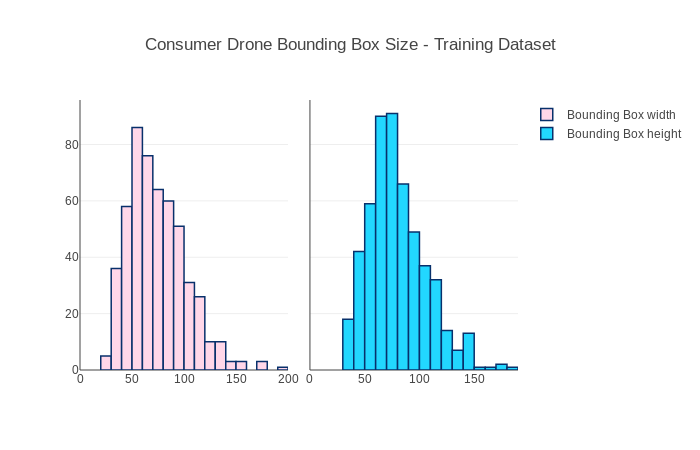
\includegraphics[scale=0.4]{images/train-histogram.png}
\caption{Consumer Drone Bounding Box Height and Width Histograms- Train data}
\end{figure}

As per qqplot show in figure \ref{consumerdronetrainqqplot} the data does not follow a normal distribution, so non-parametric tests will be performed to check that samples are obtained from the same population. 

\begin{figure}[h]
\centering
\label{consumerdronetrainqqplot}
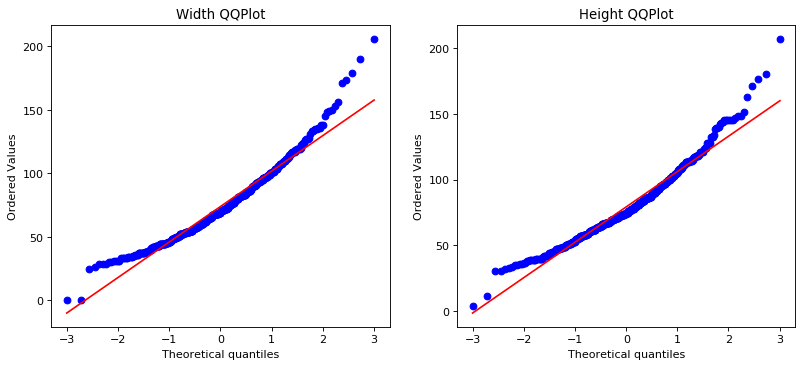
\includegraphics[scale=0.4]{images/train-qqplot.png}
\caption{Consumer Drone Bounding Box Height and Width QQplot - Train data}
\end{figure}

The aspect ratio of the training set as shown in the figure \ref{consumerdronetrainaspect} shows that there is no preference between log(-0.5) to log(0.5). This shows that there is no orientation preference of the bounding boxes in the training data set. As can be expected from aerial imagery data.

\begin{figure}[h]
\centering
\label{consumerdronetrainaspect}
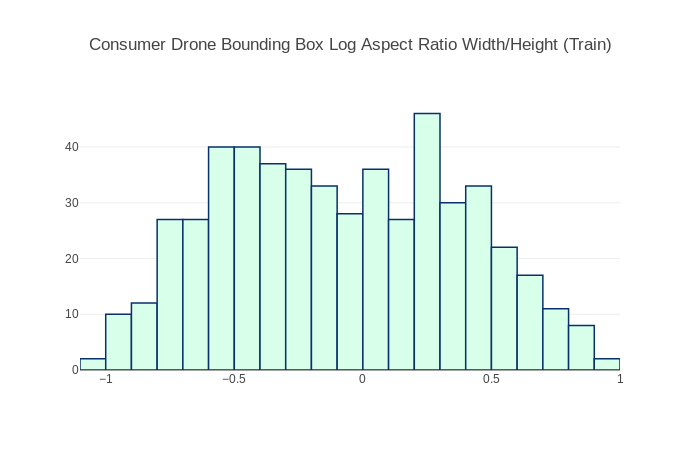
\includegraphics[scale=0.4]{images/train-aspect.png}
\caption{Consumer Drone Bounding Box Log Aspect Ratio Histogram - Train data}
\end{figure}

\section{Testing Dataset}

Testing bound boxes have a minor tendency to be larger in height than in width. The average size is also around 76 pixels, with minimum pixel size of around 29 pixels. Again this is within the field of view of the VGG16 pixel single feature vector of the \textit{conv5} output feature map. 

\begin{table}[ht]
\caption{Consumer Drone Bounding Box Statistics - Test data}
\centering
\begin{tabular}{llllll}
       & Mean   & Std. Dev. & Min & Max & Population\\
Width  & 71.654 & 29.435 & 26 & 199 & 246 \\
Height & 81.232 & 34.203 & 30 & 272 & 246
\end{tabular}
\end{table}

\begin{figure}[h]
\centering
\label{consumerdronetesthist}
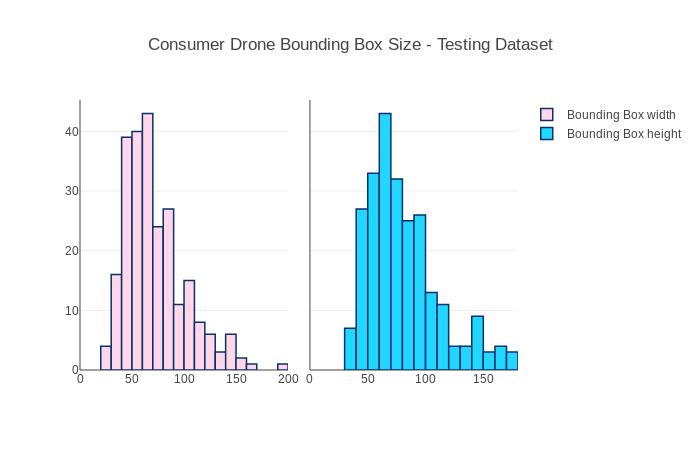
\includegraphics[scale=0.4]{images/test-histogram.png}
\caption{Consumer Drone Bounding Box Height and Width Histograms- Test data}
\end{figure}

As per qqplot show in figure \ref{consumerdronetrainqqplot} the data does not follow a normal distribution. This confirms the non-parametric tests to be performed on the population sampling.

\begin{figure}[h]
\centering
\label{consumerdronetestqqplot}
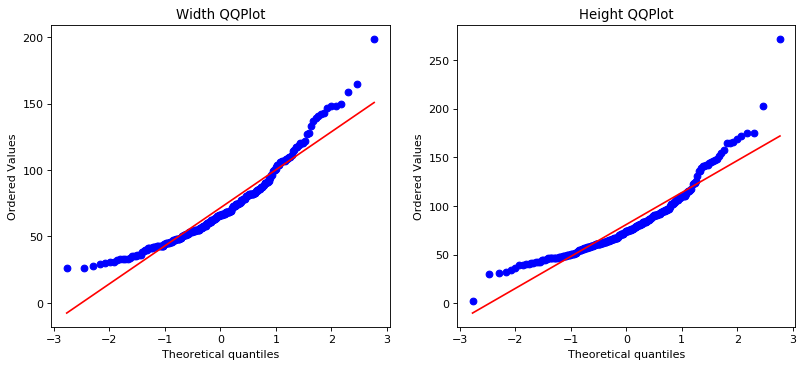
\includegraphics[scale=0.4]{images/test-qqplot.png}
\caption{Consumer Drone Bounding Box Height and Width QQplot - Test data}
\end{figure}

The aspect ratio of the training set as shown in the figure \ref{consumerdronetrainaspect} shows that there is no preference between log(-0.5) to log(0.5). This shows that there is no orientation preference of the bounding boxes in the training data set. The smaller values at the O for both the training set and the test set indicate that the objects bounding boxes are rarely a box shape (i.e. equal width and height) which indicates that the objects have an elongated shape. This is to be expected as the images labelled are of beverage bottles and containers, which are predominantly manufactured to be stacked side-by-side, and ergonomically designed to be handled by a single hand.

\begin{figure}[H]
\centering
\label{consumerdronetestaspect}
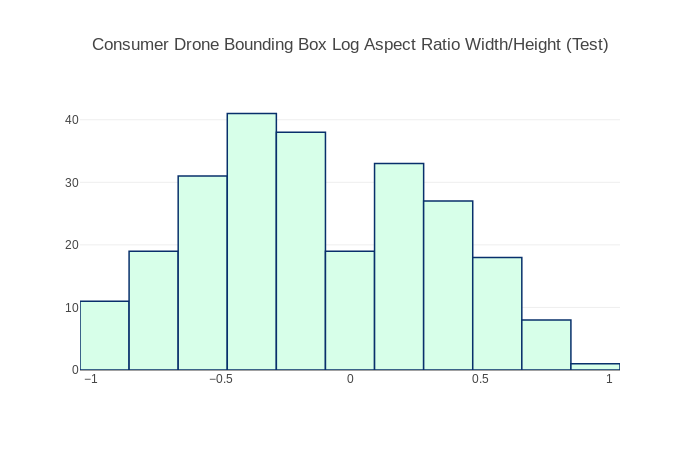
\includegraphics[scale=0.4]{images/test-aspect.png}
\caption{Consumer Drone Bounding Box Log Aspect Ratio Histogram - Test data}
\end{figure}


\section{GeoScience Dataset}

The Geoscience annotation also show no orientation prefernce with equal average width and height. The average size is also around 37 pixels, with minimum pixel size of around 11 pixels. This is a marked distinction from the previous datasets. The smaller bounding box sizes within this dataset might cause difficulties in the VGG16 field of view.

\begin{table}[ht]
\caption{GeoScience Drone Bounding Box Statistics - Data}
\centering
\begin{tabular}{llllll}
       & Mean   & Std. Dev. & Min & Max & Population\\
Width  & 36.038 & 11.921 & 11 & 120 & 793 \\
Height & 37.318 & 10.420 & 10 & 82 & 793
\end{tabular}
\end{table}

The average size of the bounding boxes of the GeoSciences is half that of the two other datasets. 

\begin{figure}[ht]
\centering
\label{geodronethist}
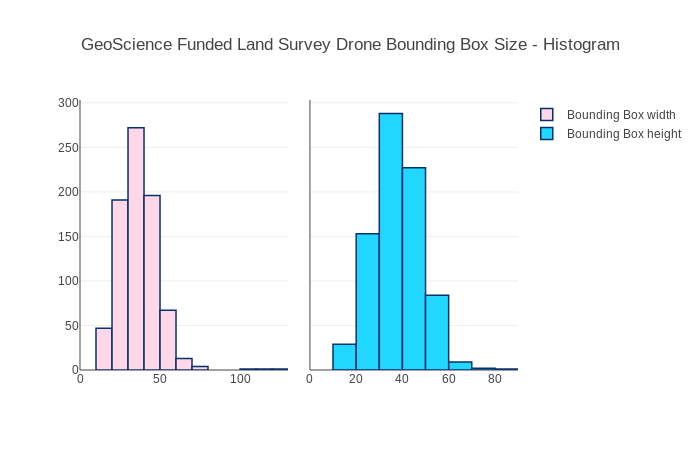
\includegraphics[scale=0.4]{images/geoscience-histogram.png}
\caption{GeoScience Bounding Box Height and Width Histograms}
\end{figure}

As per qqplot show in figure \ref{geodroneqqplot} the data does not follow a normal distribution. This confirms the non-parametric tests to be performed on the population sampling.

\begin{figure}[h]
\centering
\label{geodroneqqplot}
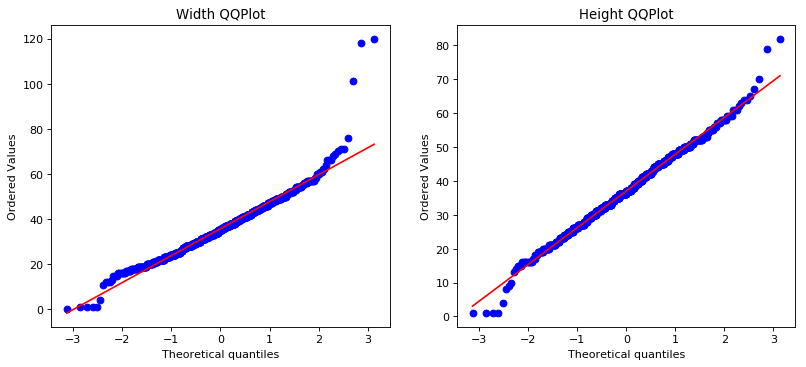
\includegraphics[scale=0.4]{images/geoscience-qqplot.png}
\caption{GeoScience Bounding Box Height and Width QQplot}
\end{figure}

The aspect ratio figure \ref{geodroneaspect} has a similar shape as the train and data set, confirming the nature of the images being labelled. 

\begin{figure}[ht]
\centering
\label{geodroneaspect}
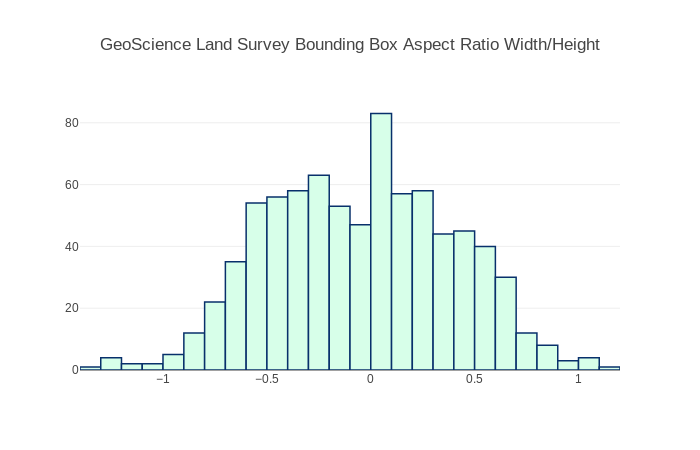
\includegraphics[scale=0.4]{images/geoscience-aspect.png}
\caption{GeoScience Bounding Box Log Aspect Ratio Histogram}
\end{figure}

\subsection{Population Testing}

The train, test and Geoscience population will be tested for independance. Since the populations are not normally distrbuted, a non-parametric test will be used. A two-tail Mann Whitney test will be performed. The whole data in the datasets will be used. The scale will be in pixel size. A confidence interval $\alpha = 0.05$ will be used.

The null hypothesis will be formulated :
\begin{nullhypothesis}
$H_0$: the distribution of the pixel sizes of the two datasets are equal
\end{nullhypothesis}
\begin{hypothesis}
$H_{A}$: the distribution of the pixel sizes is not equal
\end{hypothesis}

The two comparisons will be made between train vs test and train vs geoscience dataset.

\subsubsection{Train vs Testing Population}

Testing the two datasets using Mann Whitney results with U = 69299.00 and a p-value of 0.092 (for width) and U = 66246.50 and a p-value of 0.533 (for height) . Therefore we fail to reject the Null Hypothesis $H_0$. The train and testing data set come from the same population. This is to be expected as the data comes from the same sensor and using the same land-survey techniques.

\subsubsection{Train vs GeoScience Population}

Testing the two datasets using Mann Whitney results with U = 383029.00 and a p-value of 0.0 (for width) and U = 400391.50 and a p-value of 0.0 (for height) . Therefore we reject the Null Hypothesis $H_0$. The train and geoscience dataset come from the different populations. 

\section{Statistical Results}

The statistical tests show that the geoscience and the consumer drone data have different image sizes. This shows that the surveying techniques and parameters are different between geoscience data and consumer drone data. Comparing the geoscience images to that of the consumer drone, it can be deduced that the altitude of the surveys are different. This can also be the result of the drone operator knowledge of higher camera resolution.\newline

An algorithm which is dependant on the size of the picture for successful recognition, will have difficulty correctly infering the smaller sized dataset. The ability of the human labeller to correctly label the objects, indicates that the shape information is present. This has to be exploited by the CNN. The algorithm must be scale invariant or specifically tuned to the zoom levels of the geoscience dataset.\newline

\end{document}

